\begin{figure}[H]
  \centering
  \subfloat[Before]{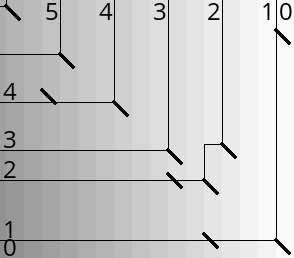
\includegraphics[width=0.4\linewidth]{imgs/fig3/start.png}\label{GLOBALfig:contours-start}}
  %\hfill
  \hspace{0.01\linewidth}
  \subfloat[After]{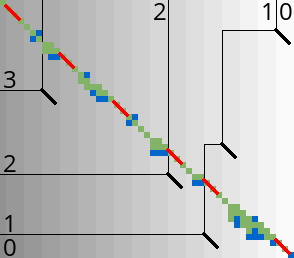
\includegraphics[width=0.4\linewidth]{imgs/fig3/end.png}\label{GLOBALfig:contours-end}}
  \caption[Execution of the chaining seed heuristic with pruning]{An example of
  the layers and contours used by the \csh before and after the \A execution
  with match pruning for $r{=}1$ and seed length $k{=}3$. Exact matches with
  ${\matchscore(m){=}1}$ are shown as black diagonal segments~(\blackmatch{}).
  \emph{Contours} are shown as horizontal and vertical black lines and indicate
  the bottom-right boundaries of \emph{layers} $\layer_\ell$ consisting of the
  states above/left of the contour marked with $\ell$. States $u$ between two
  contours have the same maximal number of matches $\cshscore(u)$ on a chain to
  the end. The value of the heuristic is shown in the background, from white
  ($h{=}0$) to darker grey.  Expanded states are shown in
  green~(\greensquare{}), open states in blue~(\bluesquare{}), and pruned
  matches in red~(\redmatch{}). Note that pruning matches during the \A
  execution shifts the contours and changes the layers. This figure is produced
  by Ragnar~Groot Koerkamp and Mykola~Akulov.}
  \label{GLOBALfig:contours}
\end{figure}
